\section[Построение модифицированной имитационной модели]{
  ПОСТРОЕНИЕ МОДИФИЦИРОВАННОЙ \\
  ИМИТАЦИОННОЙ МОДЕЛИ}
\label{sec:modified_model}

Определим параметры модели, которые могут быть подвержены модификации.
Перечислим возможные варианты:

\begin{itemize}
\item размер бункера;
\item время обработки изделий на устройствах технологической линии;
\item число параллельно работающих линий создания изделий;
\item максимальный уровень заполнения бункера, при котором происходит
  его заполнение.
\end{itemize}

Первые три варианта не подходят, так как предполагают существенное
изменения организации работы линии
(модернизация или замена бункера и/или устройств).

Последний вариант представляет собой интерес, так как не требует подобных
изменений организации работы линии.
Таким образом, в модифицированной модели мы будем изменять значение точки заказа,
т.~е. максимальный уровень заполнения бункера,
при котором происходит его заполнение.

В тексте задания не была указана зависимость между временем, которое
требуется для заполнения бункера, и текущим уровнем заполнения бункера.
На практике эти две величины часто бывают связаны функциональной зависимостью.
Поэтому для построения модифицированной имитационной модели,
учитывающей это обстоятельство, нам потребуется определить вид этой зависимости.

Предположим, что зависимость между рассматриваемыми параметрами модели
имеет линейный вид. Для определения коэффицинта наклона линейной зависимости
используем следующие соображения:

\begin{itemize}
\item по условию задачи, когда в бункере находится три килограмма 
  сырья (то есть недостаток сырья составляет 17 килограммов), 
  происходит его заполнение, которое занимает от десяти до двадцати минут
  (равномерный закон распределения);  
\item в случае, когда бункер полон,
  заполнять его не требуется, поэтому время заполнения равно нулю.
\end{itemize}

Для имитации величин, распределенных по равномерному закону, в языке GPSS
применяется функция \textbf{UNIFORM}, которая принимает в качестве аргументов 
значения нижней и верхней границы генерируемых величин.
Поэтому для отражения рассматриваемой зависимости нам потребуется определить 
две функции: \textbf{TIME\_MIN} и \textbf{TIME\_MAX},
предназначенные для определения нижней и верхней границы времени заполнения
бункера, приведенные на рисунке~\ref{lst:func_time}.

\begin{lstlisting}[caption=Функции определения верхней и нижней временной границы заполнения бункера,
label=lst:func_time,numbers=none,resetmargins=true,xleftmargin=0mm,
xrightmargin=0mm]
TIME_MIN FUNCTION    X$ZAPAS,C2
0,11.76/20,0
TIME_MAX FUNCTION    X$ZAPAS,C2
0,23.53/20,0
\end{lstlisting}

Данные функции используются в команде
\textbf{ADVANCE (UNIFORM(1, FN\$TIME\_MIN, FN\$TIME\_MAX))},
имитирующей заполнение бункера. 
Графики этих функций представлены на рисунке~\ref{pic:time_func}.

\begin{figure}[h!]
  \centering
  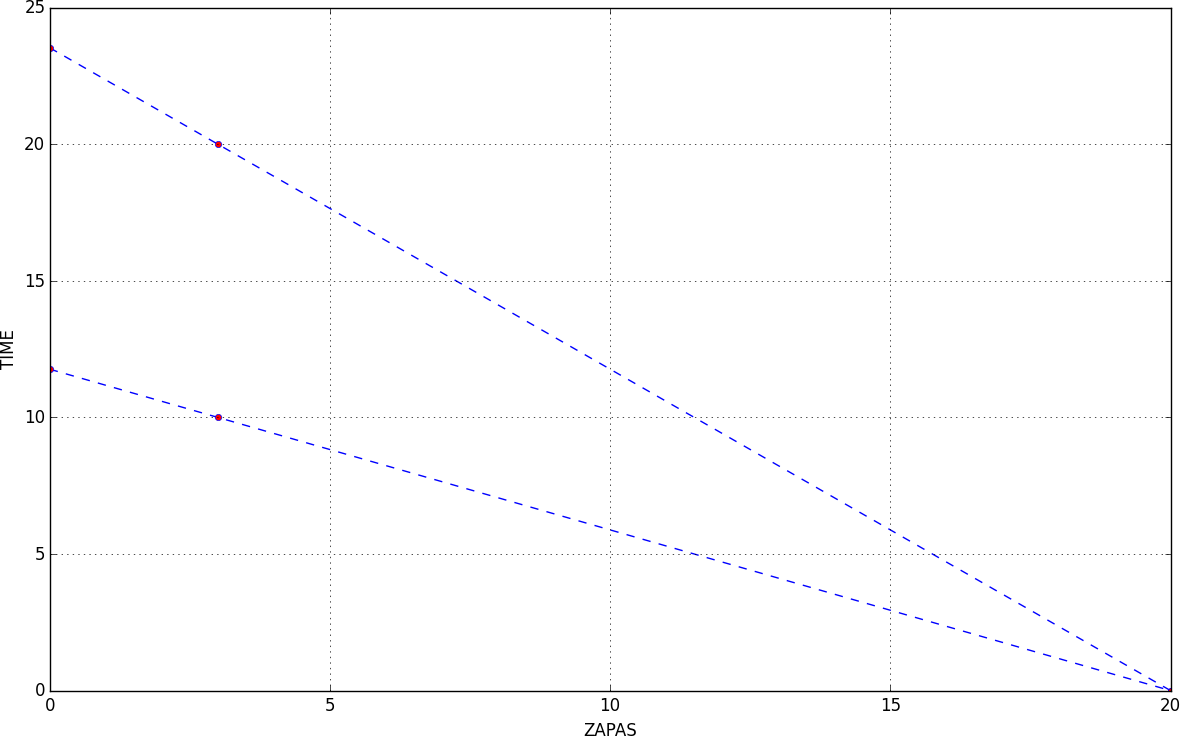
\includegraphics[width=150mm]{pic/time_func}
  \caption{Графики функций получения минимального и \\
    максимального значения времени заполнения от \\
    текущего уровня заполнения бункера}
  \label{pic:time_func}
\end{figure}


Исходный текст модифицированной GPSS-модели приведен в приложении~Б.